
\documentclass{beamer}
\usetheme{default}
\title{ATAR Notes Specialist Maths Term 1 Lecture}
\author{Stephen Zhang}

\renewcommand{\d}{\hspace{0.2cm}\text{d}}

\begin{document}

\begin{frame}
	\titlepage
\end{frame}

\begin{frame}{What's up?}
	\begin{itemize}
		\item Hope year 12 is going well for you guys =) it's been a while
		\item Take a chill pill and relax cos it's gonna be fun guys
		\item Having trouble with Specialist at this point of year? Make use of your holidays!
		\item Don't underestimate the power of \textbf{notetaking}
	\end{itemize}
\end{frame}

\begin{frame}{What's up?}
	\textbf{Notetaking}\\~\\
	Writing up \textbf{notes} for maths (and also other courses) is super important.
	\begin{itemize}
		\item Forces you to \textbf{work through} problems and derivations
		\item Don't write down a formula without understanding
	\end{itemize}
	\begin{center}
		\textbf{No point reading or listening about math ... need to work through with paper and pencil}
	\end{center}
\end{frame}

\begin{frame}{I present you this...}
	
\includegraphics[width = \linewidth]{img/quote1.png}\\
	From \textit{S. Thompson, Calculus Made Easy (1914)}
\end{frame}

\begin{frame}{So strap yourselves in...}
	\begin{center}
		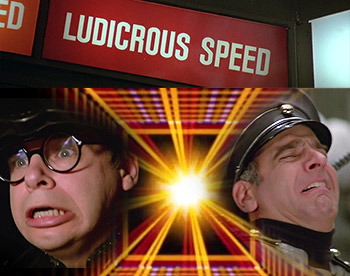
\includegraphics[scale=0.80]{img/ludicrous_speed.jpg}
	\end{center}
	\end{frame}

\section{Unit 3 recap}

\subsection{Kindergarten}
\begin{frame}
	You should recognise these formulas and know how to use them...
	\textbf{Geometric progression and series}
	\begin{itemize}
		\item $\sum_{k = 0}^{n} ar^k = a + ar + ... + ar^n = \dfrac{a(1-r^n)}{1-r}$
		\item $\sum_{k = 0}^{\infty} ar^k = a + ar + ar^2 + ... = \dfrac{a}{1-r}$\\
		$\Rightarrow$ ... under what conditions?
	\end{itemize}
	\textbf{Ellipses and hyperbolae}
	\begin{itemize}
		\item $\dfrac{x^2}{a^2} + \dfrac{y^2}{b^2} = 1 \Rightarrow \text{ellipse}$
		\item $\dfrac{x^2}{a^2} - \dfrac{y^2}{b^2} = 1 \Rightarrow \text{hyperbola... what kind?}$
		\item $\dfrac{y^2}{b^2} - \dfrac{x^2}{a^2} = 1 \Rightarrow \text{hyperbola... what kind?}$
	\end{itemize}
	Of course we can have the necessary translations: $x \to x-h$ ; $y \to y-k$.
\end{frame}

\begin{frame}
	\textbf{Example:} Plot the ellipse with equation:
	$\dfrac{x^2}{3} + \dfrac{y^2}{4} = 1$
	Hence, draw the hyperbola with equation:
	$\dfrac{x^2}{3} - \dfrac{y^2}{4} = 1$
	\vspace{5cm}
\end{frame}

\begin{frame}{Geometry}
	\begin{itemize}
		\item Circle theorems (refer to Year 11)
		\item Sine rule:
			$$\dfrac{\sin(A)}{a} = \dfrac{\sin(B)}{b} = \dfrac{\sin(C)}{c}$$
		\item Cosine rule:
			$$c^2 = a^2 + b^2 - 2ab\cos(C)$$
		\item Pythagoras theorem (and its converse)
			$$a^2 + b^2 = c^2 \Leftrightarrow \text{ABC is a right angled triangle}$$
	\end{itemize}
\end{frame}

\subsection{Vectors}
\begin{frame}{Vectors}
\begin{itemize}
	\item Recall that \textbf{vectors} are mathematical objects that are \textbf{groups} of numbers.
	\item \textbf{Vectors} are special because they satisfy a very specific set of properties - they come from \textbf{vector spaces}, e.g. $\mathbb{R}^2, \mathbb{R}^3$
	\item \textbf{Geometric interpretation:} vectors are directed line segments with a \textbf{head} and \textbf{tail}
\end{itemize}
\end{frame}

\begin{frame}{Vector toolbox}
	\begin{itemize}
		\item \textbf{Scalar multiplication: }\\$\vec{v} \to \lambda \vec{v}$ stretches $\vec{v}$ by $|\lambda|$ and possibly reverses direction.
		\item \textbf{Addition: }\\$\vec{a} + \vec{b} = \vec{b} + \vec{a}$, add head $\to$ tail
		\item \textbf{Subtraction: }\\ $\vec{a} - \vec{b} = \vec{a} + (-1)\vec{b}$
		\item \textbf{Magnitude: }\\$|\vec{a}| = \text{length of }\vec{a}$, $|\vec{a}| \ge 0$
		\item \textbf{Scalar product: }\\ $\vec{a}\cdot\vec{b} = |\vec{a}||\vec{b}|\cos(\theta)$
		\item \textbf{Unit vector: }\\ $\hat{a} = \dfrac{\vec{a}}{|\vec{a}|}$
	\end{itemize}
\end{frame}

\begin{frame}{Vector toolbox}
	\begin{center}
	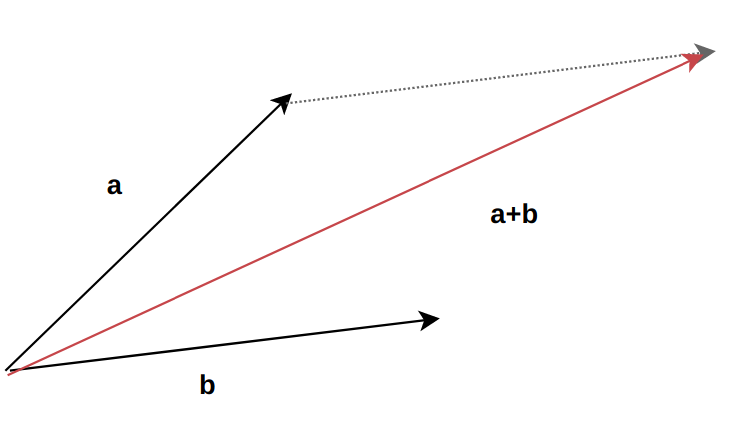
\includegraphics[width = 0.75\linewidth]{img/vector_addition.png}
	\end{center}
\end{frame}

\begin{frame}{Vector toolbox}
	\textbf{Scalar product}\\~\\
	The scalar ($\equiv$ dot) product between two vectors is super useful.
	
	$$\vec{u} \cdot \vec{v} = |\vec{u}||\vec{v}|\cos(\theta)$$
	
	In fact, the \textbf{scalar product} is what defines the concept of \textbf{distance} and \textbf{orientation} in our vector space.
	\\~\\
	For instance, the magnitude of a vector is formally defined as:
	
	$$|\vec{u}| = \sqrt{\vec{u}\cdot\vec{u}}$$
	
	The scalar product we are using is the \textbf{Euclidean} inner product. There are other strange beasts out there, though.
\end{frame}

\begin{frame}{Vector toolbox}
	\textbf{Vector projections}
	Given two vectors $\vec{a}, \vec{b}$, we can consider $\vec{a}_\parallel$, the projection of $\vec{a}$ onto $\vec{b}$
	$$\vec{a}_\parallel = \left(\dfrac{\vec{a}\cdot\vec{b}}{\vec{b}\cdot\vec{b}}\right)\vec{b} = (\vec{a}\cdot\hat{b})\hat{b}$$
	\begin{center}
	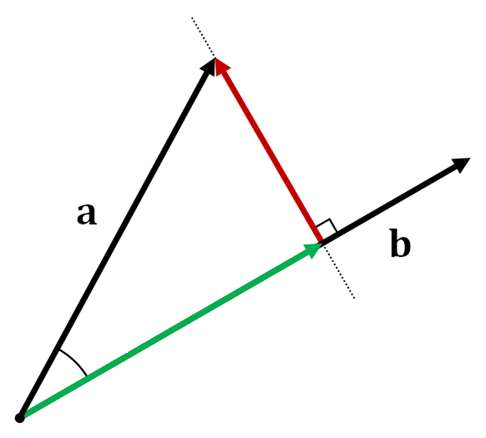
\includegraphics[width=0.50 	\linewidth]{img/vector_projection.png}
	\end{center}
\end{frame}

\begin{frame}{Vector toolbox}
	\textbf{Vector projection}
	Once we have $\vec{a}_\parallel$, $\vec{a}_\perp$ can simply be found by subtracting:
	
	$$\vec{a}_\perp = \vec{a} - \vec{a}_\parallel$$
	
	\begin{center}
	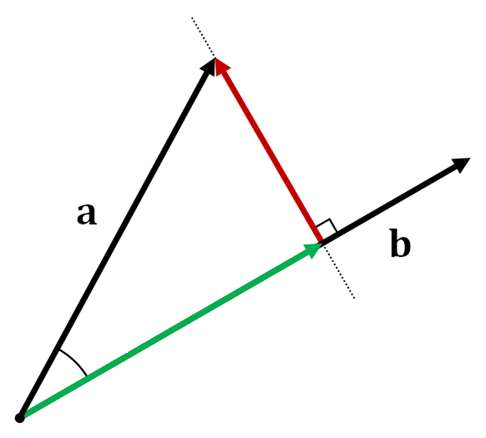
\includegraphics[width=0.50 	\linewidth]{img/vector_projection.png}
	\end{center}
\end{frame}

\begin{frame}{Ratio theorem}
	This is an important theorem...
	$$\vec{r} = \dfrac{\mu\vec{a} + \lambda \vec{b}}{\lambda + \mu}$$
	\begin{center}
	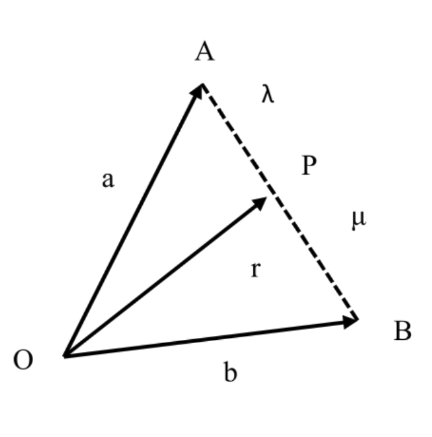
\includegraphics[scale = 0.40]{img/ratio_theorem.png}
	\end{center}
\end{frame}

\begin{frame}{Cartesian representation}
	We've been speaking about vectors in an abstract manner. In $\mathbb{R}^2, \mathbb{R}^3$, we can \textbf{project} a vector $\vec{a}$ onto a \textbf{basis} $\{\vec{i}, \vec{j}, \vec{k}\}$
	\begin{align*}
		\vec{a} &= (\vec{a}\cdot\vec{i})\vec{i} + (\vec{a}\cdot\vec{j})\vec{j} + (\vec{a}\cdot\vec{k})\vec{k}\\
				&= a_1\vec{i} + a_2\vec{j} + a_3\vec{k}\\
				&= (a_1, a_2, a_3)\\
	\end{align*}
	
	We say that $a_1, a_2, a_3$ are \textbf{projections} of our vector $\vec{a}$ in the $x, y, z$ directions respectively. Can we derive this from our previous definitions of \textbf{vector projections}?
\end{frame}

\begin{frame}{Cartesian representation}
	Using the \textbf{Cartesian representation} of vectors, we find that:
	\begin{itemize}
		\item \textbf{Scalar multiplication: } $\lambda(a_1, a_2, a_3) = (\lambda a_1, \lambda a_2, \lambda a_3)$
		\item \textbf{Addition: } $(a_1, a_2, a_3) + (b_1, b_2, b_3) = (a_1 + b_1, a_2 + b_2, a_3 + b_3)$
		\item \textbf{Magnitude: } $|(a_1, a_2, a_3)| = \sqrt{a_1^2 + a_2^2 + a_3^2}$
		\item \textbf{Scalar product: } $(a_1, a_2, a_3)\cdot(b_1, b_2, b_3) = a_1b_1 + a_2b_2 + a_3b_3$
	\end{itemize}
\end{frame}

\begin{frame}{Pythagoras in 3D}
	We said previously that
	$$|\vec{a}| = \sqrt{a_1^2 + a_2^2 + a_3^2}$$
	
	This is \textbf{Pythagoras' theorem} for 3 dimensions. Proof?
	\begin{center}
		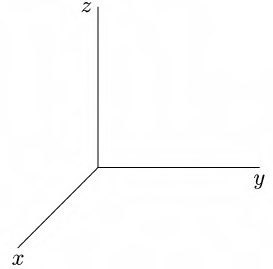
\includegraphics[scale = 0.5]{img/axes.png}
	\end{center}
\end{frame}

\begin{frame}
	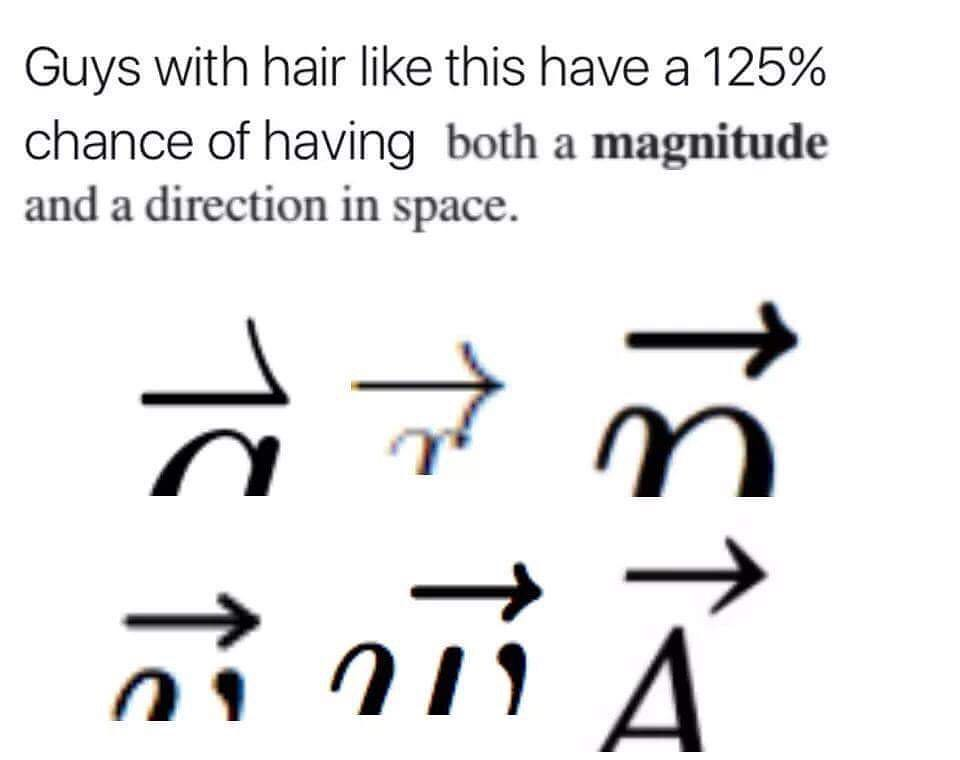
\includegraphics[width = \linewidth]{img/vector_meme.jpg}
\end{frame}

\begin{frame}{Linear independence}
	\textbf{Any} set of vectors will either be linearly \textbf{dependent} or otherwise \textbf{independent}.
	
	\textbf{Formal definition}
	
	$\vec{a}, \vec{b}, \vec{c}$ are \textbf{linearly dependent} if there exists $k_1, k_2, k_3$ \textbf{not all zero} such that:
	
	$$k_1\vec{a} + k_2\vec{b} + k_3\vec{c} = \vec{0}$$
	
	\textbf{Practical definition}
	
	$\vec{a}, \vec{b}, \vec{c}$ are \textbf{linearly dependent} if we can write \textbf{one vector} as a \textbf{linear combination} of the others.
	
	E.g. $\vec{c} = m\vec{a} + n\vec{b}$, and so on.
\end{frame}

\begin{frame}{Linear independence}
	\begin{align*}
		\vec{a} &= \vec{i} + 3\vec{j} + \vec{k}\\
		\vec{b} &= -2\vec{j} + 5\vec{k}\\
		\vec{c} &= 2\vec{i} + 17\vec{k}
	\end{align*}
	
	$\{\vec{a}, \vec{b}, \vec{c}\}$ are \textbf{linearly dependent} since
	$\vec{c} = 2\vec{a} + 3\vec{b}$
\end{frame}

\begin{frame}{Linear independence}
	If a set of vectors is \textbf{not} linearly dependent, then it is \textbf{linearly independent}.
	
	\textbf{Useful special cases:}
	\begin{itemize}
		\item 2 vectors are dependent only if they are \textbf{parallel}
		\item In 2 dimensions, any set of $>$2 vectors will be dependent
		\item In 3 dimensions, any set of $>$3 vectors will be dependent
		\item Any 3 \textbf{coplanar} vectors will be dependent
	\end{itemize}
\end{frame}

\begin{frame}
	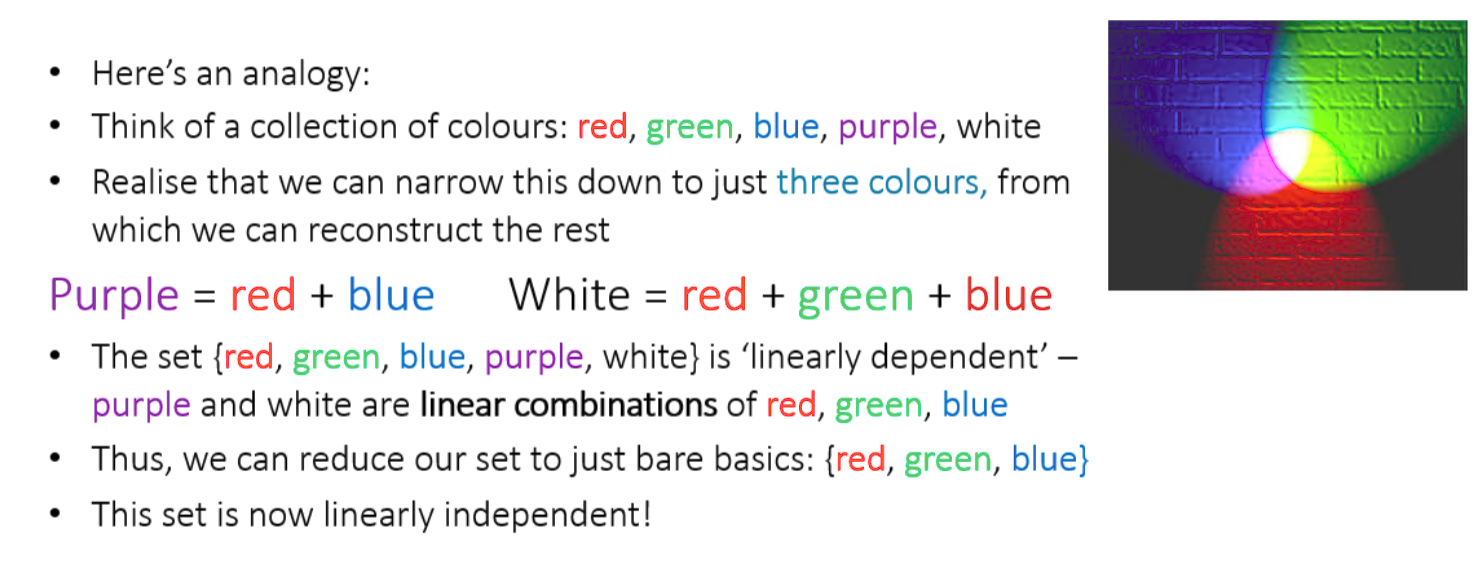
\includegraphics[width = \linewidth]{img/indep_1.png}
\end{frame}

\begin{frame}
	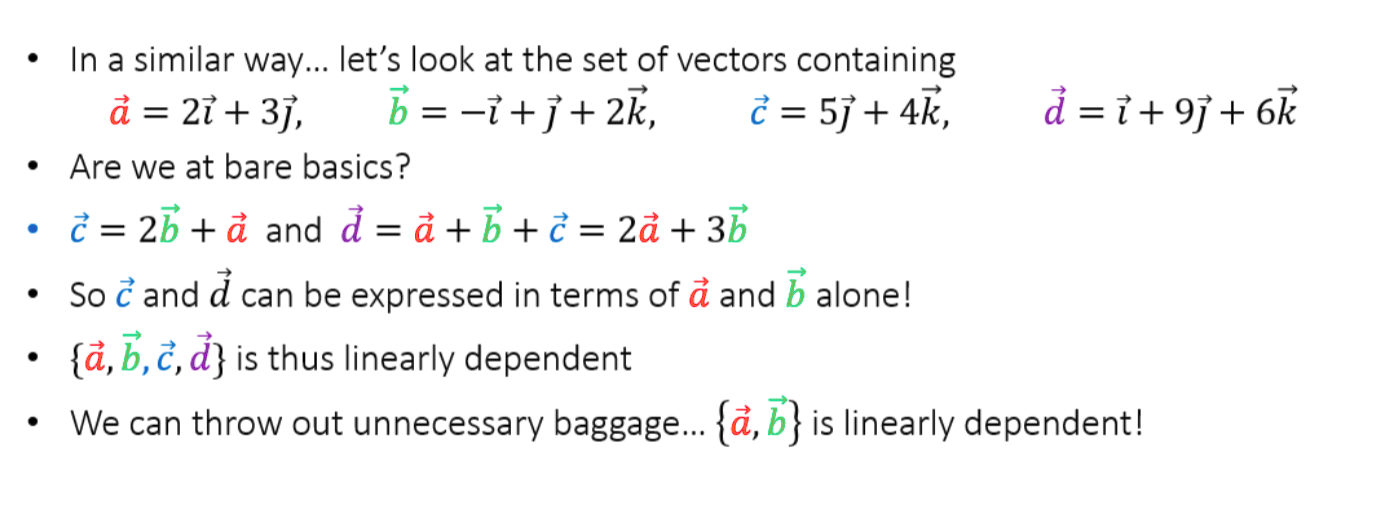
\includegraphics[width = \linewidth]{img/indep_2.png}
\end{frame}

\begin{frame}
	Example: VCAA 2009 Exam 2
	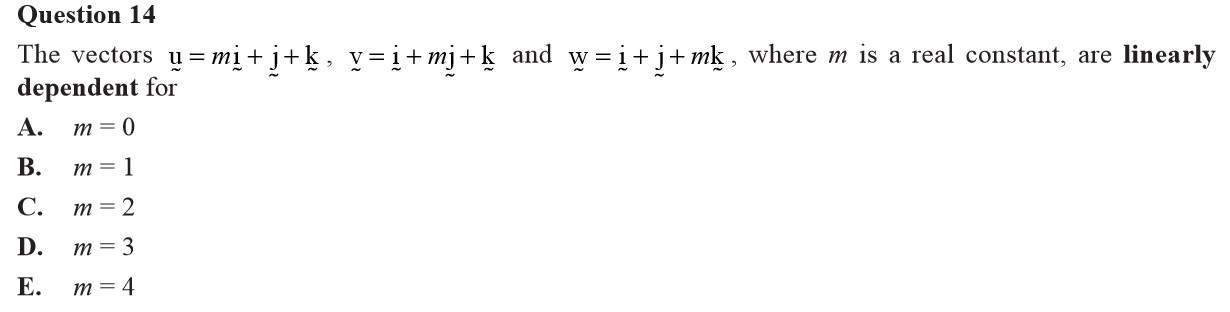
\includegraphics[width = \linewidth]{img/q1.png}
\end{frame}

\begin{frame}
	Example: VCAA 2009 Exam 1
	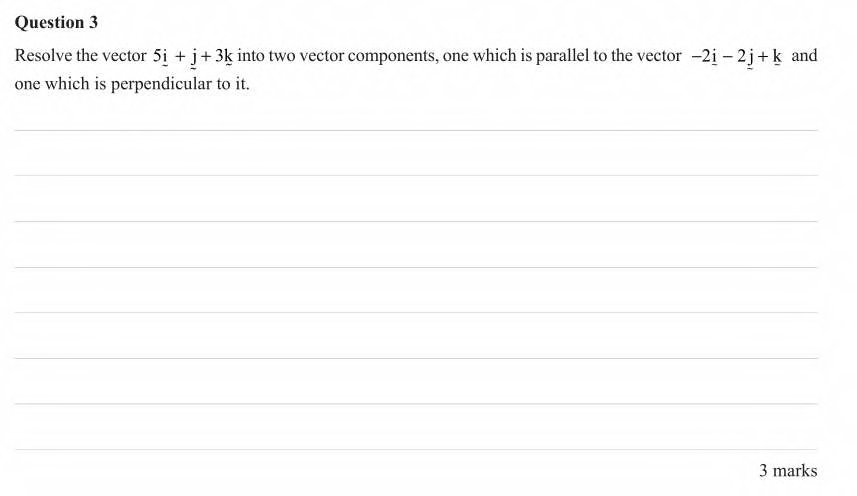
\includegraphics[width = \linewidth]{img/q2.png}
\end{frame}

\begin{frame}

	\textbf{Challenge problem}
	\\~\\
	Using vector projections, find the point on the line $y = 3x - 2$ that is closest to the point $(4, 2)$. 
	What is the minimal distance between the point $(4, 2)$ and the line?	
	
	\vspace{5cm}
	
	% (8/5, 14/5), and distance is 4sqrt(10)/5

\end{frame}

\section{Complex numbers}

\begin{frame}{Complex numbers basics}
	\textbf{Definition of a complex number...}
	
	$$\mathbb{C} = \{z = x + iy : x, y \in \mathbb{R} \}$$
	
	
	\textbf{Complex numbers} follow the basic arithmetic and algebraic properties we are used to applying to \textbf{reals}.
	\\~\\
	\textbf{However}, we do have some extras...

\end{frame}

\begin{frame}{Complex conjugate}
	The \textbf{conjugate} of a complex number $z$ is denoted $\bar{z}$, and:
	
	$$z = x + iy \Rightarrow \bar{z} = x - iy$$
	
	The conjugate satisfies some \textbf{very important} properties...
	\begin{itemize}
		\item $z\bar{z} = (x + iy)(x - iy) = |z|^2$
		\item $z + \bar{z} = 2\mathrm{Re}(z)$
		\item $z - \bar{z} = 2i\mathrm{Im}(z)$
		\\~\\
		\item $\overline{z + w} = \bar{z} + \bar{w}$
		\item $\overline{zw} = \bar{z}\bar{w}$
		\item $\overline{z/w} = \bar{z}/\bar{w}$
	\end{itemize}
	
	
\end{frame}

\begin{frame}{Polar form}
	Complex numbers can be expressed in \textbf{polar form} - this makes multiplication, division and exponentiation a lot easier.
	
	$$z = r\mathrm{cis}(\theta) = r(\cos(\theta) + i \sin(\theta))$$
	\vspace{5cm}
	
	We write $r = |z|$ and $\theta = \mathrm{arg}(z)$
\end{frame}

\begin{frame}{Polar form}
	\textbf{Polar form} makes some things much easier...
	\begin{itemize}
		\item $z_1 z_2 = r_1 r_2 \mathrm{cis}(\theta_1 + \theta_2)$
		\item $z_1/z_2 = \dfrac{r_1}{r_2}\mathrm{cis}(\theta_1 - \theta_2)$
		\item $z^n = r^n \mathrm{cis}(n\theta) \quad \leftarrow \quad \text{De Moivre's Theorem}$
	\end{itemize}
\end{frame}

\begin{frame}
	\textbf{Problem.} Find in \textbf{Cartesian form}: $u = \mathrm{cis}(\pi/4), v = \mathrm{cis}(\pi/3)$.\\~\\
	Hence, find the values of $\sin(\pi/12)$ and $\cos(\pi/12)$
	\vspace{5cm}
\end{frame}

\begin{frame}{Factorisation over $\mathbb{C}$}
	\textbf{Fundamental Theorem of Algebra (formal statement)}\\
	Every polynomial in $P$ in $z$:
	$$P(z) = a_n z^n + a_{n-1}z^{n-1} + ... + a_2 z^2 + a_1 z + a_0$$
	where $a_n \ne 0$ and $a_0, ..., a_n \in \mathbb{C}$ has at least \textbf{one} linear factor in $\mathbb{C}$.
	\\~\\
	\textbf{Version for p l e b s:}\\
	Any polynomial of degree $n$ will have $n$ linear factors over $\mathbb{C}$.
\end{frame}

\begin{frame}
	\textbf{Quadratics: } we typically \textbf{complete the square}... best shown by example.
	\\~\\
	Factorise $z^2 + 3z + 4$
	\vspace{5cm}
	\\
	For higher order polynomials typically you'll need to use the \textbf{remainder theorem} to reduce to a quadratic
\end{frame}

\begin{frame}
	\textbf{Problem: } VCAA 2014 Exam 1
	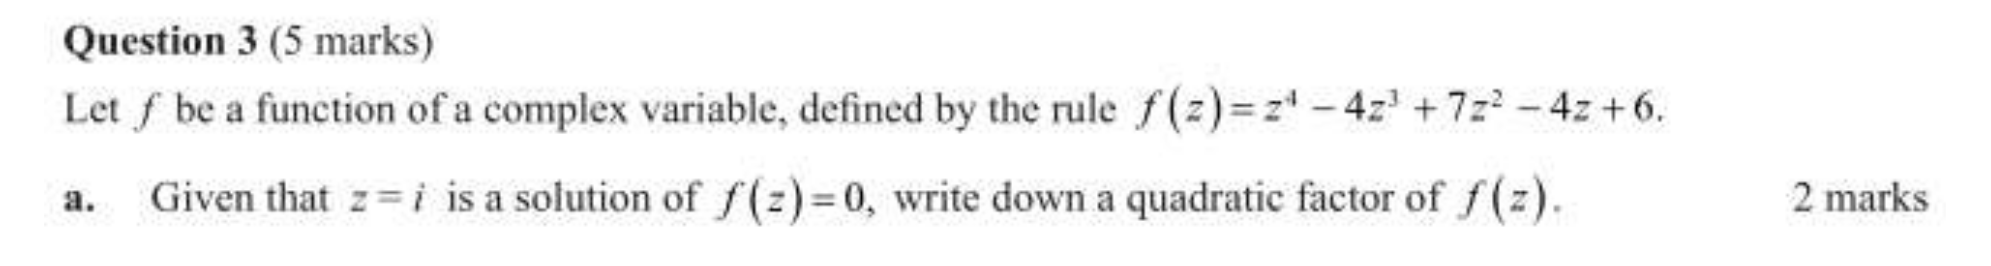
\includegraphics[width=\linewidth]{img/q3a.png}
	\vspace{4cm}
\end{frame}

\begin{frame}
	\textbf{Problem: } VCAA 2014 Exam 1
	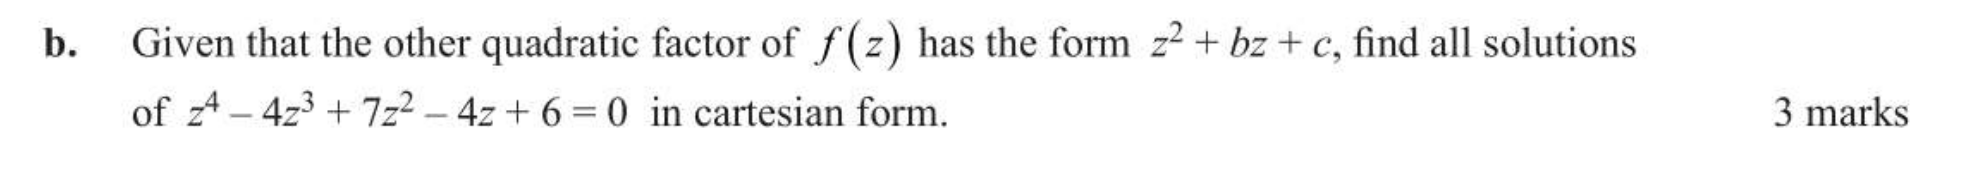
\includegraphics[width=\linewidth]{img/q3b.png}
	\vspace{4cm}
\end{frame}

\begin{frame}{plz don't kill me for this}
	\begin{center} who would win??!!!1111 \end{center}

	\begin{align*}
		&\text{An irreducible quadratic}\quad\quad\quad\quad&\text{one dreamy boi}\\
		& z^2 + 2x + 2 & z = x + iy
	\end{align*}	
\end{frame}

\begin{frame}{$n$th roots}
	We can find the $n$th roots of any complex number using de Moivre's Theorem in the following procedure...
	
	$$z^n = a, n \in \mathbb{N}$$
	
	\begin{itemize}
		\item There will be $n$ solutions $w_1, ..., w_n$ (c.f. Fundamental Theorem of Algebra)
		\item Solutions will lie on the circle with radius $|a|^{1/n}$ at even intervals of $2\pi/n$.
	\end{itemize}
\end{frame}

\begin{frame}
	\textbf{Example:} find the fourth roots of unity.
	\vspace{5cm}
\end{frame}

\begin{frame}
	\begin{center}
	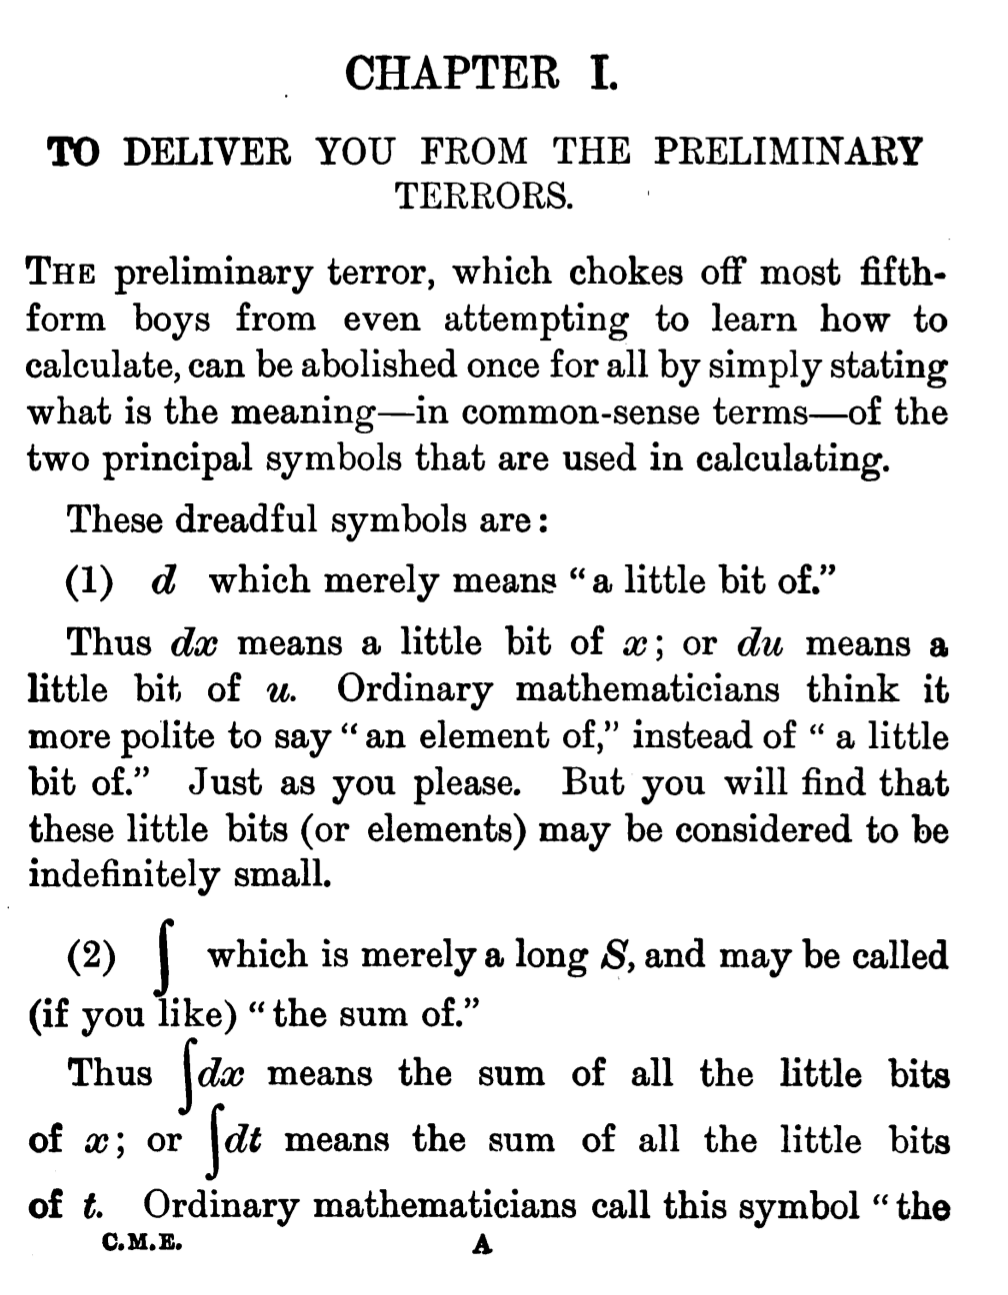
\includegraphics[width=0.5\linewidth]{img/quote2.png}
	\end{center}
	From \textit{S. Thompson, Calculus Made Easy (1914)}
\end{frame}

\begin{frame}{Differentiation}
	\textbf{Assumed knowledge: } most of Methods calculus. For those of you who haven't seen...
	\begin{align*}
		\dfrac{d}{dx} \sin(x) &= \cos(x)\\
		\dfrac{d}{dx} \cos(x) &= -\sin(x)\\
		\dfrac{d}{dx} \tan(x) &= \sec^2(x)\\
		\dfrac{d}{dx} \ln(x) &= \dfrac{1}{x}\\
		\dfrac{d}{dx} e^x &= e^x
	\end{align*}
	
	Also the \textbf{chain rule}:
	
	$$\dfrac{dy}{dx} = \dfrac{dy}{dt} \dfrac{dt}{dx}$$
	
\end{frame}

\begin{frame}{A few new functions...}
	You will have encountered already...
	\begin{align*}
		\arcsin(x) &= \sin^{-1}(x)\\
		\arccos(x) &= \cos^{-1}(x)\\
		\arctan(x) &= \tan^{-1}(x)
	\end{align*}

We seek their \textbf{derivatives...}

\begin{align*}
	\arcsin'(x) &= \dfrac{1}{\sqrt{1-x^2}}\\
	\arccos'(x) &= \dfrac{-1}{\sqrt{1-x^2}}\\
	\arctan'(x) &= \dfrac{1}{1+x^2}
\end{align*}
\end{frame}

\begin{frame}
	Let's derive these ...
	
	$$\arctan'(x) = \dfrac{1}{1+x^2}$$
	
	Let $y = \tan(x), \quad x \in (-\pi/2, \pi/2), \quad y \in \mathbb{R}$. Thus $x = \arctan(y)$.
	\vspace{5cm}
\end{frame}

\begin{frame}{The modulus function}
	You've probably seen already the modulus function...
	$$|x| = x\mathrm{sgn(x)} = \text{'positive value of x'}$$
	
	From the graph of $|x|$ we see that our function is \textbf{continuous everywhere}, and \textbf{differentiable} away from the origin.
	
	\begin{center}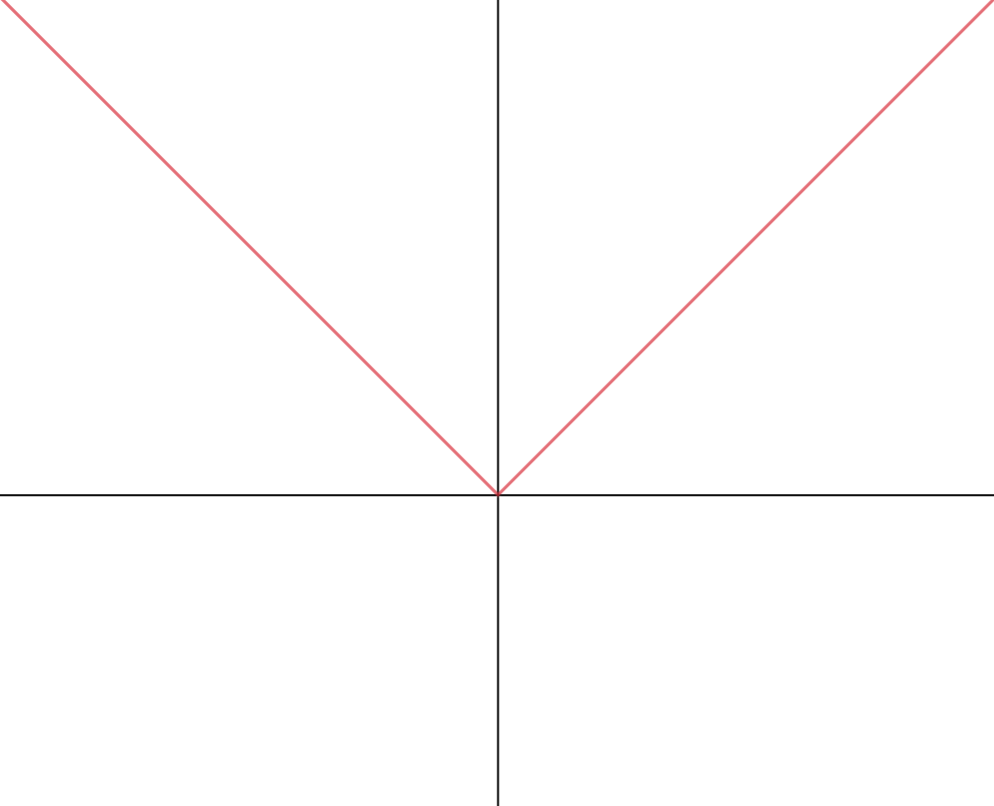
\includegraphics[scale=0.10]{img/abs.png}\end{center}
	
	$$\dfrac{d}{dx} |x| = \begin{cases}+1, x > 0\\ -1, x < 0\end{cases}$$
\end{frame}

\begin{frame}{Implicit differentiation}
	So far, we have been able to differentiate expressions where $y$ is \textbf{explicitly} related to $x$.
	\\~\\	
	Implicit relations allow us to find derivatives where $y$ and $x$ are \textbf{implicitly} tangled together... 
	\begin{center}for example in the expression $x \cos(y) + y\cos(x) = 1$\end{center}
	
	\textbf{Quick rule: } to find $dy/dx$, differentiate as per usual w.r.t $x$, using chain/product/quotient rules as required, but write 
	$$\dfrac{d}{dx}(y) = \dfrac{dy}{dx} \quad \text{(obviously!!!)}$$
\end{frame}

\begin{frame}
	\textbf{Example:} given that $x \cos(y) + y \cos(x) = 1$, find an expression for $dy/dx$.
	\vspace{5cm}
\end{frame}

\begin{frame}
	Here's a cheap way to do the same thing...\\~\\
	To differentiate some relation, rearrange into the form $F(x, y) = 0$ and then find \textbf{partial derivatives} $F_x, F_y$. From this, we have:
	
	$$\dfrac{dy}{dx} = -\dfrac{F_x}{F_y}$$

	\begin{itemize}
		\item To find $F_x$, differentiate $F(x, y)$ w.r.t $x$, treating $y$ like a \textbf{constant}
		\item To find $F_y$, differentiate $F(x, y)$ w.r.t $y$, treating $x$ like a \textbf{constant}
	\end{itemize}
\end{frame}

\begin{frame}{Concavity and the second derivative test}
	\begin{itemize}
		\item We know that \textbf{stationary points} can be a local \textbf{maximum}, \textbf{minimum}, or \textbf{point of inflection}
		\item \textbf{Without} sketching a graph, how would we be able to classify stationary points of a graph?
		\item We first introduce the idea of \textbf{concavity}
	\end{itemize}
\end{frame}

\begin{frame}{Concavity}
	\textbf{Concavity} of a curve at a given point tells us whether the curve is 'curving upwards' or 'curving downwards'
	\begin{itemize}
		\item Consider the second derivative $f''(x) = \dfrac{d^2f}{dx^2}$
		\item \textbf{Case: } $f''(x) > 0$ $\Rightarrow$ concave up (slope is increasing)
		\item \textbf{Case: } $f''(x) < 0$ $\Rightarrow$ concave down (slope is decreasing)
		\item \textbf{Case: } $f''(x) = 0$ $\Rightarrow$ zero concavity, i.e. locally our curve has no 'curvature'
	\end{itemize}
\end{frame}

\begin{frame}{Second derivative test}
	Thus, given a \textbf{stationary point} at $x = x_0$, we can check the value of $f''(x_0)$ to determine the type of stationary point.
		
	\begin{itemize}
		\item $f''(x_0) > 0$ $\Rightarrow$ concave up $\Rightarrow$ local minimum
		\item $f''(x_0) < 0$ $\Rightarrow$ concave down $\Rightarrow$ local maximum
		\item $f''(x_0) = 0$ $\Rightarrow$ no concavity $\Rightarrow$ inconclusive
	\end{itemize}
	
	This is the \textbf{second derivative test.}
\end{frame}


\begin{frame}{Second derivative test}
	\textbf{What if $f''(x_0) = 0$?}
	\\~\\
	If $f''$ \textbf{switches sign} around $x_0$...
	\begin{itemize}
		\item We know that $y = f(x)$ changes its concavity around $x_0$
		\item Thus $y = f(x)$ has a \textbf{point of inflection} at $x_0$
		\item Depending on whether $f'(x_0) = 0$\\	this could be a \textbf{stationary point of inflection}\\or a \textbf{non-stationary point of inflection}
	\end{itemize}
\end{frame}

\begin{frame}{Second derivative test}
	\textbf{What if $f''(x_0) = 0$?}
	\\~\\
	In other cases, we actually \textbf{can't make any conclusions}!
	\begin{itemize}
		\item Consider $y = x^4$ and $y = x^5$.
		\item \textbf{Both} of these satisfy $dy/dx = d^2y/dx^2 = 0$ at $x = 0$
		\begin{itemize}
			\item $y = x^4$ has a local minimum
			\item $y = x^5$ has an inflection.
			
		\end{itemize}
		\item \textbf{Thus}, in general we will need \textbf{further investigation} in these cases
	\end{itemize}	
\end{frame}

\begin{frame}{Second derivative test}
	\textbf{Problem}: find and classify all the stationary points of $y = x^2 e^{-x}$
	\vspace{5cm}
\end{frame}

\begin{frame}{Integration techniques}
	We will follow on from what we learned in Methods.\\~\\
	\textbf{Definition of antiderivative}\\~\\
	For a (sufficiently nice) function $f(x)$, we say $F(x)$ is an antiderivative of $f$ if
	$$\dfrac{dF}{dx} = f$$
\end{frame}

\begin{frame}{Integration techniques}
	\textbf{Connection between definite integrals and the antiderivative}\\~\\
	$$\int_a^b f(x) dx = F(b) - F(a)$$
	Where $F$ is \textbf{any} antiderivative of $f$.\\~\\
	Our definite integral itself can be interpreted as the (signed) area bounded by $f$ and the $x$-axis on the interval $[a, b]$
\end{frame}

\begin{frame}{Substitution of variables}
	This is a very powerful technique that allows us to compute \textbf{indefinite integrals} ($\equiv$ antiderivatives) of a wide range of functions.
	\\~\\
	Consider an integral of the general form:
	$$\int u'(t) f(u(t)) dt$$
	
	We can make a substitution $v = u(t) \Rightarrow dv = u'(t) dt$
	This brings us to
	
	$$\int u'(t) f(u(t)) dt = \int u'(t) f(u(t)) \dfrac{dv}{u'(t)} = \int f(v) dv$$
\end{frame}

\begin{frame}{Substitution of variables}
	\textbf{Problem: } Compute $$\int x e^{x^2} dx$$
	\vspace{5cm}
\end{frame}

\begin{frame}{Substitution of variables}
	\textbf{Problem: } Compute $$\int \dfrac{3 \d x}{x \ln^2(x)}$$
	\vspace{5cm}
\end{frame}

\begin{frame}{Substitution of variables}
	We can also perform substitution of variables for \textbf{definite integrals} - we just need to also substitute the terminals.
\end{frame}

\begin{frame}{Substitution of variables}
	\textbf{Problem (VCAA 2017 Exam 1):} Find $$\int_1^{\sqrt{3}} \dfrac{dx}{x(1+x^2)}$$
	\vspace{5cm}
\end{frame}

\begin{frame}{Integration of trig functions}
\textbf{Important identities}
\begin{itemize}
	\item $\cos^2(x) = \dfrac{1 + \cos(2x)}{2}$
	\item $\sin^2(x) = \dfrac{1 - \cos(2x)}{2}$
	\item $\sin(2x) = 2\sin(x)\cos(x)$
\end{itemize}

\textbf{Example: } $\displaystyle\int \sin^2(x)\cos^2(x) \d x$

\end{frame}

\end{document}